In this section, we summarize the \deflateblock format~\cite{RFC1951} to explain the issue of backward pointers hindering parallelization and to explain our block finder optimizations.
We also give a short description of the two-stage \deflate decompression.

\subsection{The Deflate Stream Format}

\begin{figure}
    \centering
    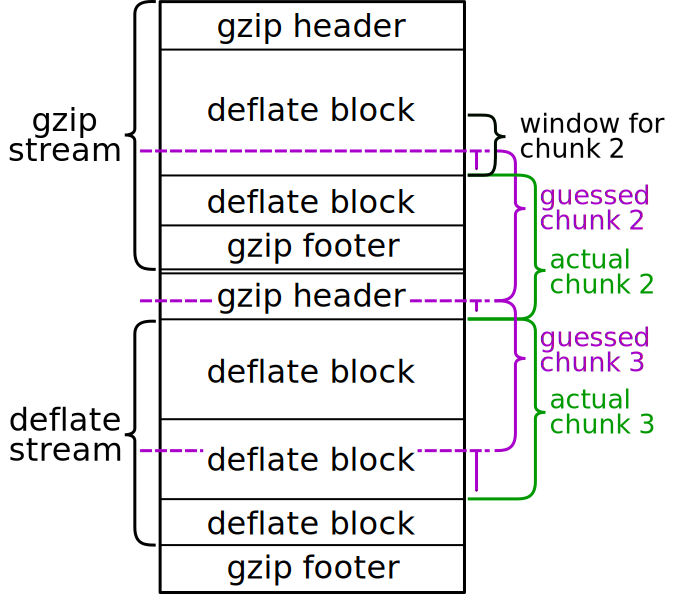
\includegraphics[width=0.5\linewidth]{figures/gzip-file}
    \caption{
        The structure of a gzip file. Also marked are the chunks as they are assigned to the decompression threads and the first \deflateblock in each chunk, i.e, the actual chunk start as it will be written to the index.
    }
    \label{fig:gzip-file}
\end{figure}

Even though the presented parallel decompressor works on gzip files, most implementation details are focused on the \deflate format.
The gzip file format~\cite{RFC1952}, shown in \cref{fig:gzip-file}, consists of one or more gzip streams.
A gzip stream wraps a raw \deflate stream and adds metadata such as file format identification bytes, the original file name, and a checksum.

\begin{figure}
    \centering
    \begin{minipage}{0.49\linewidth}\begin{center}
        \textbf{\rawblock}\\[8pt]
        \includegraphics[scale=1]{figures/non-compressed-deflate-block.pdf}\\[8pt]
        \textbf{\fixedblock}\\[10pt]
        \includegraphics[scale=1]{figures/fixed-huffman-coding-deflate-block.pdf}
    \end{center}\end{minipage}\begin{minipage}{0.49\linewidth}\begin{center}
        \textbf{\dynblock}\\[8pt]
        \includegraphics[scale=1]{figures/dynamic-huffman-coding-deflate-block.pdf}
    \end{center}\end{minipage}
    \caption{
        Deflate block formats.
        A \deflateblock can start at any bit offset.
        \rawblocks add padding bits after the block type to byte-align the length fields and the subsequent data.
        The block is the last one in the \deflate stream if the final-block (BF) bit is set.
        The block type value $\mathbf{{11}_2}$ is reserved.
    }
    \label{fig:deflate_blocks}
\end{figure}

\Cref{fig:deflate_blocks} shows the three types of \deflate blocks:
\begin{itemize}
    \item Non-Compressed: Contains a stream of original data. Used for incompressible data.
    \item Compression with fixed Huffman codes: Contains data compressed with a predefined \huffcode.
          Used for small data to save space by not storing a custom \huffcode.
    \item Compression with dynamic Huffman codes: Contains a \huffcode in its header followed by data compressed with it.
\end{itemize}
These blocks will be referred to in shortened forms as \rawblock, \fixedblock, and \dynblock.
\deflate blocks are concatenated to a \deflate stream without any byte-alignment.

Each \dynblock uses three different Huffman codes (HC): one is for the Literal alphabet, the second one for the Distance alphabet, and the third one is to encode the code lengths (CL) for defining the first two Huffman codes themselves also referred to as Precode.
The size of each HC is stored in HLIT, HDIST, and HCLEN respectively as shown in \cref{fig:deflate_blocks}.

The steps for decompressing a \dynblock are as follows:
\begin{enumerate}
    \item Read the lengths HLIT, HDIST, and HCLEN.
    \item Read the code lengths for the Precode and build a Huffman code from them.
    \item Use the \huffcode defined by the Precode to read the code lengths for the Distance alphabet and the Literal alphabet.
    \item Build a Huffman code from the Distance alphabet code lengths.
    \item Build a Huffman code from the Literal alphabet code lengths.
    \item Decode the \deflate data using the Literal and Distance alphabets.
\end{enumerate}

The compressed data encoded with the Literal alphabet contains either raw literals or pointers to duplicated strings, i.e., instructions to copy a given length of data from a given distance.
The distance is limited to \SI{32}{\kibi\byte} of decompressed data, i.e., backward pointers are limited to a sliding window.
Small lengths are encoded in the instructions and large lengths require reading more bits from the stream.
A distance encoded using the Distance \huffcode follows all backward pointers.

The instructions to copy sequences from the \backrefwindow introduce data dependencies that complicate parallelization.



\subsection{Two-Stage Deflate Decoding}
\label{sct:theory:two-stage-decompression}

\begin{figure}
    \centering
    \includegraphics[width=0.95\linewidth]{figures/two-stage-decompression.pdf}
    \caption{Example of \deflate compression and two-stage decompression.}
    \label{fig:two-stage-example}
\end{figure}

The authors of \pugz~\cite{pugz} show that it is feasible to parallelize decompression even if there are instructions to copy from an unknown \backrefwindow.
This is done by resolving placeholders for unknown values in a second step after those values have become known.
An example of this two-stage decompression is shown in~\cref{fig:two-stage-example}.
The steps for a decompression thread starting at an arbitrary offset in the file are:
\begin{enumerate}
    \item Find the next \deflateblock.
          Searching for \deflate blocks is a technique that has previously been used for reconstructing corrupted gzip files~\cite{park2008data}.
          This can be implemented by trying to decompress at the given offset and going to the next offset on error.
    \item Start decoding by filling the as-of-yet unknown \backrefwindow with unique 15-bit wide markers corresponding to the offset in the buffer.
          The decompression routine has to be adjusted to output an intermediate format with 16-bit symbols to store the markers itself or a literal and an additional bit to signal whether it is a marker or a literal.
    \item After the \backrefwindow has become available, replace all marker symbols with data from the \backrefwindow to get the fully decompressed contents.
\end{enumerate}

The benchmark results in \cref{sct:evaluation} show that the marker replacement is a magnitude faster than \deflate decompression.
This means that even if only the first stage has been parallelized and the marker replacement is applied serially, then decompression would be up to a magnitude faster. %
The \backrefwindows can be propagated even faster because the marker replacement only has to be applied for the last \SI{32}{\kibi\byte} of each chunk.
The remaining marker symbols can be replaced in parallel such that each chunk is processed by a different thread.
The propagation of the windows cannot be parallelized.
Assuming a chunk size of \SI{4}{\mebi\byte}, propagating only the last \SI{32}{\kibi\byte} of each chunk would be \num{128} times faster than replacing the markers in the whole chunk.
However, the non-parallelizable part takes up half the time when using \num{128} cores.
Therefore, the maximum achievable speedup depends on the chunk size and has an upper bound according to Amdahl's law.
